% Dies ist Teil der Vorlesung Physik auf dem Computer, SS 2012,
% Axel Arnold, Universitaet Stuttgart.
% 
% Dieses Werk ist unter einer Creative Commons-Lizenz vom Typ
% Namensnennung-Weitergabe unter gleichen Bedingungen 3.0 Deutschland
% zugänglich. Um eine Kopie dieser Lizenz einzusehen, konsultieren Sie
% http://creativecommons.org/licenses/by-sa/3.0/de/ oder wenden Sie sich
% schriftlich an Creative Commons, 444 Castro Street, Suite 900, Mountain
% View, California, 94041, USA.

% !TEX root = padc.tex

\chapter{Datenanalyse und Signalverarbeitung}

In diesem Kapitel geht es darum, was man mit einem gemessenen Signal
machen kann und muss. Ein gemessenes Signal kann dabei entweder
tatsächlich von einem Messgerät kommen oder aber das Ergebnis einer
Computersimulation sein. Zwei Fragen sind dabei vor allem wichtig:
Welche Eigenschaften hat das Signal, und wie vertrauenswürdig sind die
Werte?

Um die Eigenschaften von Signalen zu untersuchen, ist die
kontinuierliche Fourieranalyse ein gutes Werkzeug, die das Signal vom
Zeit- in den Frequenzraum überträgt. So lassen sich zum Bespiel
charakteristische Frequenzen und damit Zeitskalen bestimmen. Außerdem
bietet der Übergang in den Frequenzraum analytisch viele Vorteile, die
sich auch auf dem Computer nutzen lassen. So werden zum Beispiel
langreichweitige Wechselwirkungen in Molekulardynamiksimulationen
meist im Frequenzraum berechnet.

Als weiteres Werkzeug werden wir Faltungen kennen lernen, die
erlauben, Signale nach bestimmten Frequenzen zu filtern oder aber aus
der (gemessenen) Antwort eines linearen Systems auf ein einfaches
Eingangssignal die Antwort auf beliebige Signale zu berechnen.

Sollen Signale mit dem Computer weiterverarbeitet werden, müssen diese
\emph{digitalisiert} werden, also in eine Reihe von Zahlen
übersetzt. Üblicherweise passiert dies dadurch, dass das Signal nur zu
äquidistanten Zeitpunkten ausgewertet, \emph{abgetastet} wird. Das
wirft die Frage auf, welche Funktionen dadurch überhaupt gut gemessen
werden können. Wie wir sehen werden, beschränkt diese Abtastung die
Frequenzen, die von einer digitalen Auswertung erfasst werden können.

Die meisten Signale sind außerdem, durch Messungenauigkeiten und
prinzipielle stochastische Prozesse, selbst \emph{stochastisch},
\dh die Verteilung der Ergebnisse vieler Messungen ist
vorherbestimmbar, die einzelne Messung hingegen nicht. Trotzdem sind
Messungen oft korreliert, zum Beispiel weil eine Observable sich nur
kontinuierlich ändert.  Durch Korrelationsanalysen lässt sich
bestimmen, wann Messungen wirklich unabhängig sind. Dies gibt wiederum
Aufschluss über die Zeitskalen wichtiger Prozesse im System, ist aber
auch wichtig für eine korrekte Abschätzung des Messfehlers, womit sich
der letzte Abschnitt beschäftigt.

\section{Kontinuierliche Fouriertransformation}
\index{Fouriertransformation>kontinuierliche}

Für die Analyse zeitlich veränderlicher Signale besonders nützlich ist
die Fouriertransformation, die ein kontinuierliches Signal in den
Frequenzraum übersetzt. Dies gilt nicht nur für periodische Signale,
sondern zum Beispiel auch dann, wenn die Antwort eines Systems auf ein
komplexes Eingangssignal gefragt ist. Der tiefere Grund dafür ist,
dass die Fouriertransformation Differential- und Integraloperatoren in
einfache algebraische Operationen übersetzt.

Betrachten wir nochmals die Fourierreihe im Interval $[-T/2,T/2)$
\begin{multline}
  f(t) = \sum_{n\in\ZZ}
  \left(\frac{\Delta\omega}{2\pi}\int_{-T/2}^{T/2}
    f(t)e^{-i n\Delta\omega t}\, dt\right)
  e^{i n\Delta\omega t}\\
  =
  \frac{1}{\sqrt{2\pi}}\sum_{n\in\ZZ}
  \left(\frac{1}{\sqrt{2\pi}}\int_{-T/2}^{T/2} f(t)e^{-i \omega t}\,dt\right)
  e^{i \omega t}\,\Delta\omega
\end{multline}
mit der Grundfrequenz $\Delta\omega=2\pi/T$ und
$\omega=n\Delta\omega$. Im Grenzwert $T\to\infty$ ergibt sich
\begin{equation}
  \label{eq:contfourierinverse}
  f(t) = \frac{1}{\sqrt{2\pi}}\int_{-\infty}^{\infty}
  \FT(f)(\omega)e^{i \omega t}\,d\omega
\end{equation}
mit
\begin{equation}
  \label{eq:contfourier}
  \FT(f)(\omega) =
  \frac{1}{\sqrt{2\pi}}\int_{-\infty}^{\infty} f(t)e^{-i \omega t}\, dt.
\end{equation}
Die \emph{kontinuierliche Fouriertransformation} $\FT$ ist das
Analogon der periodischen Fourierreihe, ist allerdings keine
Transformation in eine Reihe mehr, sondern eine Abbildung zwischen
Funktionen. Für $\FT$ gelten eine Menge sehr starker Aussagen, die wir
zum großen Teil in ähnlicher Art schon von der Fourierreihe kennen:
\begin{itemize}
\item $\FT(f)$ existiert, falls $f$ quadratintegrabel ist, und
  bildet $f$ auf eine quadratintegrable Funktion ab. Für solche
  Funktionen mit der zugehörigen Norm $\lVert f \rVert_2 =
  \int_{-\infty}^{\infty} \lvert f(t) \rvert^2\,dt$ gilt dann sogar
  die Isometrie
  (\emph{Parsevaltheorem}\index{Parsevaltheorem>kontinuierliches}):
  \begin{equation}
    \lVert \FT(f) \rVert_2 = \lVert f \rVert_2
  \end{equation}
\item $\FT$ ist linear, \dh $\FT(f + \lambda g) = \FT{f} + \lambda
  \FT{g}$.
\item $\FT$ ist reziprok gegen Streckungen, \dh
  \begin{equation}
    \label{eq:fourierreziprok}
    \FT[f(\alpha
    t)](\omega) = \frac{1}{\lvert \alpha \rvert}
    \FT(f)\left(\frac{\omega}{\alpha}\right).
  \end{equation}
  Wird also eine Funktion $\alpha$ immer stärker gestaucht, so wird
  ihre Transformierte immer weiter gestreckt.  Entsprechend wird aus
  Zeitumkehr Frequenzumkehr: $\FT(f(-t))(\omega) = \FT(f)(-\omega)$.
\item $\FT$ ist invertierbar, die Umkehrfunktion $\FT^{-1}$ ist durch
  \eqref{eq:contfourierinverse} explizit gegeben. Offenbar ist auch
  die Umkehrung eine Isometrie, es gilt $\lVert \FT^{-1}(f)
  \rVert_2 =\lVert f \rVert_2$.
\item Weiter gilt $\FT(\FT(f(t))) = f(-t)$, und damit $\FT^4(f) =
  f$. Insbesondere ist auch $\FT^{-1} = \FT^3$. Die
  Fouriertransformation ist damit eine vierte Einheitswurzel auf dem
  Raum der quadratintegrablen Funktionen, ähnlich wie $i$ bei den
  komplexen Zahlen.
\item Eine zeitliche Verschiebung wird zu einer Frequenzmodulation und
  umgekehrt:
  \begin{eqnarray}
    \label{eq:fouriertimeshift}
    \FT(f(t-t_0))(\omega) = e^{-i\omega t_0} \FT(f(t))(\omega)\\
    \label{eq:fourierfreqshift}
    \FT(e^{i\omega_0 t}f(t))(\omega) = \FT(f(t))(\omega-\omega_0).
  \end{eqnarray}
  Wird also ein niederfrequentes Signal (Radioprogramm) auf ein
  hochfrequentes Trägersignal aufmoduliert, verschiebt sich nur dessen
  Spektrum. 
\item Aus der Linearität folgt, dass stets gilt:
  $\FT(\overline{f})(\omega) = \overline{\FT(f)(\omega)}$.
\item Ist Funktion $f$ gerade (symmetrisch), also $f(t) = f(-t)$, so ist
  $\FT(f)(-\omega) = \FT(f)(\omega)$, also gerade (symmetrisch).
\item Ist Funktion $f$ ungerade (antisymmetrisch), also $f(t) = -f(-t)$, so ist
  $\FT(f)(-\omega) = -\FT(f)(\omega)$, ungerade (antisymmetrisch).
\item Ist Funktion $f$ reellwertig, also $f(t) = \overline{f(t)}$, so
  ist $\FT(f)(-\omega) = \overline{\FT(f)(\omega)}$, aber im
  allgemeinen komplexwertig!
\item Für die Fouriertransformierte der Ableitung gilt
  \begin{equation}
    \begin{split}
      \FT\left(\frac{d}{dt}f(t)\right)(\omega) &=
      \frac{1}{\sqrt{2\pi}}\int_{-\infty}^{\infty}
      \left[\frac{df}{dt}(t)\right]e^{-i
        \omega t}\, dt\\
      &\substack{=\\\text{part. Int.}} -\frac{1}{\sqrt{2\pi}}\int_{-\infty}^{\infty}
      f(t)\frac{d}{dt}e^{-i \omega t}\, dt = i\omega
      \FT(f(t))(\omega).
    \end{split}
  \end{equation}
  Dies spielt eine wichtige Rolle beim Lösen von
  Differenzialgleichungen, weil diese in gewöhnliche algebraische
  Gleichungen übergehen.
\item Es gilt die Poissonsche Summenformel
  \begin{equation}
    \label{eq:poissonsumme}
    \sum_{k\in\ZZ}f(t_0 + k\, \delta)=
    \frac{\sqrt{2\pi}}{|\delta|}\sum_{n\in\ZZ}\FT(f)
    \left(\frac{2\pi n}{\delta}\right)
    \exp\left(i \frac{2\pi n}{\delta} t_0\right).
  \end{equation}
  Diese Gleichung beruht darauf, dass $\sum_{t\in\ZZ}f(\cdot + t\,
  \delta)$ eine $\delta$-periodische Funktion ist, die durch eine
  Fourierreihe dargestellt werden kann. Wegen
  \eqref{eq:fouriertimeshift} reicht es
  dabei o.B.d.A. $\delta=1$ zu
  betrachten:
  \begin{multline}
    \sum_{k\in\ZZ}f(t_0 + k) =
    \sum_{n\in\ZZ} \int_0^1 \sum_{k\in\ZZ}f(\tau + k)e^{-2\pi i
      n \tau}\, d\tau
    \, e^{2\pi i n t_0} =\\
    \sum_{n\in\ZZ} \int_{-\infty}^\infty f(\tau)e^{-2\pi i
      n \tau}\, d\tau
    \, e^{2\pi i n t_0}
    = \sqrt{2\pi}\sum_{n\in\ZZ}\FT(f)(2\pi n)\, e^{2\pi i n t_0}.
  \end{multline}

  Eine wichtige Anwendung der Poissonschen Summenformel ist die
  Summation schlecht konvergenter Reihen. Fällt die Funktion $f$ sehr
  langsam gegen unendlich ab, so fällt ihre Fouriertransformierte
  wegen der Reziprozität \eqref{eq:fourierreziprok} im Allgemeinen
  schneller, so das aus einer langsam eine rasch konvergierende Reihe
  wird.
\end{itemize}

\subsection{Spezielle Fouriertransformierte}

Die Fouriertransformierte einer Gaußglocke ist
\begin{equation}
  \FT\left(\frac{1}{\sqrt{2\pi}}e^{-t^2/2}\right)
  =
  \frac{1}{2\pi}e^{-\omega^2/2}\int_{-\infty}^{\infty} e^{-(t-i\omega)^2/2}\, dt
  =
  \frac{1}{\sqrt{2\pi}}e^{-\omega^2/2}
\end{equation}
Die Gaussglocke ist also eine Eigenfunktion der Fouriertransformation
zum Eigenwert 1. Die Fouriertransformation hat tatsächlich sehr viel
mehr echt verschiedene Eigenfunktionen, die Familie der
Hermitefunktionen~\cite{pinsky02a}. Wegen $\FT^4=1$ kann die
Fouriertransformation nur die vier Eigenwerte $\pm 1$ und $\pm i$
haben. Jeder dieser Eigenwerte ist stark degeneriert, also der
Eigenraum zu jedem Eigenwert unendlichdimensional.

Die (formale) Fouriertransformierte der $\delta$-Funktion ist
\begin{equation}
  \label{eq:fourierdelta}
  \FT(\delta(t))(\omega)
  =
  \frac{1}{\sqrt{2\pi}}\int_{-\infty}^{\infty}
  \delta(t)e^{-i \omega t}\, dt = \frac{1}{\sqrt{2\pi}},
\end{equation}
also einfach die konstante Funktion $1/\sqrt{2\pi}$, die ebensowenig
wie die $\delta$-Funktion eine quadratintegrable Funktion
ist. Alternativ lässt sich die Beziehung aus der
Fouriertransformierten der Gaußglocke mit sinkender Varianz herleiten.

\subsection{Numerische kontinuierliche Fouriertransformation}
\label{sec:contdft}

\begin{figure}
  \centering
  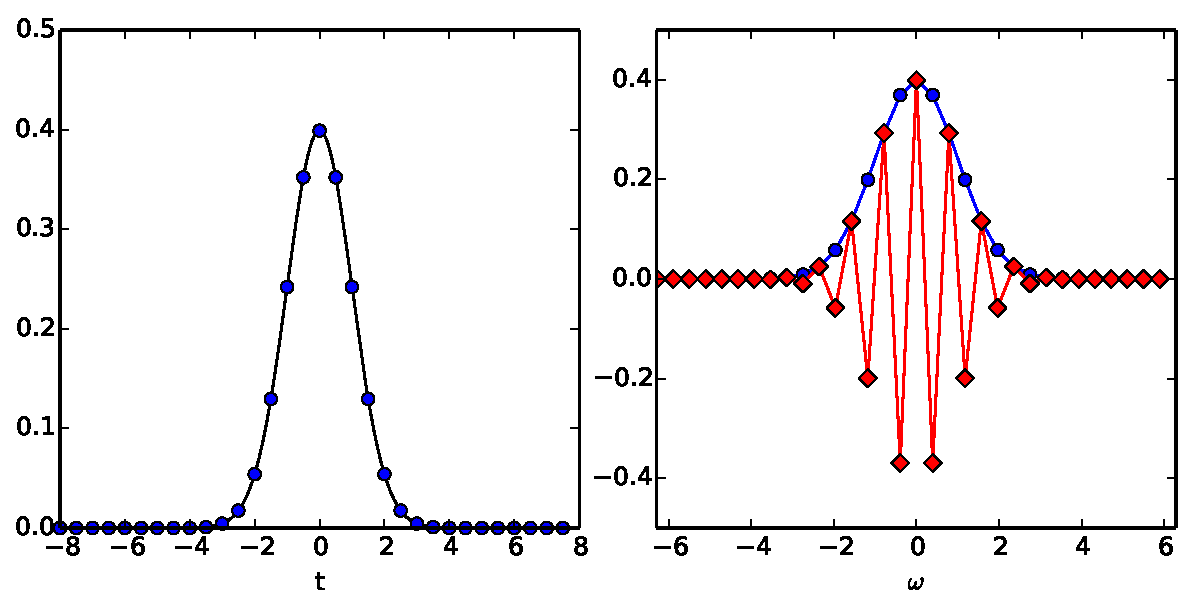
\includegraphics[width=\textwidth]{plots/dft}
  \caption{Numerische kontinuierliche Fouriertransformation einer
  Gaußglocke $g(t) = e^{-t^2/2}$, die wie links gezeigt äquidistant
  an den Stützstellen $t_k=-8 + k/2$, $k=0(1)31$ diskretisiert wird.
  Werden die gewonnenen Daten $g(t_k)$ diskret fouriertransformiert,
  ergibt sich als Transformierte eine Gaußglocke mit wechselnden
  Vorzeichen, wie rechts mit blauen Kreisen gezeigt. Nur mit dem
  notwendigen Phasenshiftfaktor $e^{-2\pi i 8/16}=-1$ erhält man die
  erwartete Gaußglocke (rote Rauten).}
  \label{fig:contdft}
\end{figure}

Um die Eigenschaften der kontinuierlichen Fouriertransformation
numerisch zu nutzen, machen wir den Grenzübergang $T\to\infty$
rückgängig und ziehen uns auf ein für die betrachtetete Funktion
hinreichend großes $T$ zurück, so dass $\int_{\lvert t\rvert>T}\lvert
f(t)\rvert^2\, dt$ hinreichend klein ist. Das geht insbesondere, wenn
das Signal endlichen Träger hat, wie das bei echten gemessenen
Signalen stets der Fall ist.

Wir betrachten nun als Signal eine Funktion $f$, die wir nur an auf
einem äquidistanten Gitter $t_k = t_0 + k\frac{T}{N}$, $k=0(1)N-1$
kennen, also im Intervall $[t_0, t_0 + T)$. Dann setzen wir
$\omega_0:=\frac{2\pi}{T}$ und $\Delta := \frac{T}{N}$, und erhalten
für ganzzahliges $n$
\begin{multline}
  \label{eq:dftcont}
  \FT(f)(\omega_0 n)\approx
  \frac{1}{\sqrt{2\pi}}\int_{t_0}^{t_0 + T} f(t)e^{-i n \omega_0 t}\, dt
  \approx
  \frac{1}{\sqrt{2\pi}}\sum_{k=0}^{N-1}
  \Delta f(t_k)
  e^{-i n\omega_0 \left(t_0 + k\Delta\right)}\,
  \\
  =   \Delta \frac{e^{-i n\omega_0 t_0}}{\sqrt{2\pi}}\sum_{k=0}^{N-1}
  f(t_k) e^{-2\pi i n k / N}\,
  =\frac{T}{N}\frac{\left(e^{-i\omega_0 t_0}\right)^n}{\sqrt{2\pi}} \text{DFT}(f(t_k))_n\,,
\end{multline}
wobei DFT die diskrete Fouriertransformation aus \eqref{eq:dft}
bezeichnet. Meist werden Messungen bei $t=0$ begonnen, die Funktion
ist dann nur im positiven Halbinterval von Null verschieden.  In
diesem Fall wählt man natürlicherweise $t_0 = 0$, so dass der Phasenfaktor
$e^{-i\omega_0 t_0} = 1$ entfällt. Wir werden allerdings später noch
Faltungen kennenlernen, bei denen es häufig natürlicher ist, eine
symmetrische Lage der Filterfunktion um die Null anzunehmen. In diesem
Fall wählt man $t_0 = -T/2$, so dass $e^{-i\omega_0 t_0} = -1$.

Um die Rolle des Phasenfaktors zu illustrieren, betrachten wir eine
Gaußglocke, die wir an um die Null symmetrisch liegenden Stützstellen diskretisieren. Wie wir gesehen hatten, ist die Fouriertransformierte
der Gaußglocke die Gaußglocke selber. Abbildung~\ref{fig:contdft} zeigt,
das wir diese Transformierte nur mit dem Phasenfaktor erhalten. Da
dieser gerade $(-1)^n$ beträgt, wechselt die Transformierte sonst andauernd
das Vorzeichen. Insbesondere würde mit steigender Anzahl Stützstellen das
Vorzeichen immer rascher wechseln, die Transformierte also nicht einmal
konvergieren.

Die Koeffizienten der DFT sind periodisch, daher auch diese Näherung
für $\FT(f)$. Tatsächlich sollten die Koeffizienten aber nur als
Frequenzen im Interval $[-\omega_0 N/2,\omega_0 N/2]$ interpretiert
werden, alle Frequenzen außerhalb dieses Intervals sollten als Null
angesehen werden. Der Grund dafür ist das Abtasttheorem, dass im
folgenden Abschnitt besprochen wird. Dieses besagt, dass bei einem
Zeitschritt $\Delta=T/N$ nur Kreisfrequenzen bis $\omega_0 N/2 =
\pi/\Delta$ eindeutig gemessen werden können. Daher ist die
Beschränkung auf das innerste Intervall die natürliche
Interpretation. Bei rein reellen Signalen sollte man daher
die reellen Varianten der FFT-Implementationen benutzen, die
nur die relevanten positiven Koeffizienten bis $N/2$
zurückgeben.

Die Einschränkung der Frequenzen ist besonders wichtig, wenn $N$
ungerade ist und die um Null symmetrische Lage von $-T/2$ bis $T/2$
gewählt wird. Dann ist $\left(e^{-i\omega_0 t_0}\right)^{N-n} =
(-1)^{N-n} = - (-1)^{-n} = -\left(e^{-i\omega_0 t_0}\right)^{-n}$. Mit
anderen Worten, wird einfach die gesamte diskrete
Fouriertransformierte mit $(-1)^n$ multipliziert, so bekommen die
negativen Frequenzen das falsche Vorzeichen. Das hat drastische
Konsequenzen: wenn die Ursprungsfunktion reell ist, gilt
$DFT(f_k)_{-n}=\overline{DFT(f_k)}_{n}$, für die genäherte
kontinuierliche Fouriertransformierte also
$\FT(f)(-\omega)=-\overline{\FT(f)(\omega)}$. Das entspricht der
Tranformierten einer rein imaginären Funktion!

Analog wie die Fouriertransformation selber lässt sich auch ihre
Rücktransformation nähern:
\begin{equation}
  \label{eq:idftcont}
  \FT^{-1}(f)(t_k)\approx
  \text{iDFT}\left(\sqrt{2\pi}\frac{N}{T}\left(e^{i\omega_0 t_0}\right)^n f_n\right)_k
\end{equation}
Der Faktor $\left(e^{i\omega_0 t_0}\right)^n$ invertiert genau den
Faktor $\left(e^{-i\omega_0 t_0}\right)^n$ der
Vorwärtstransformation. Für $t_0=0$ ist er wieder 1 und muss nicht
berücksichtigt werden, bei $t_0=-T/2$ ist er $(-1)^n$.

Die bekannten schnellen FFT-Routinen lassen sich also auch für die
numerische Bearbeitung der kontinuierlichen Fouriertransformation
nutzen. Auf diese Weise ist \zb Abbildung~\ref{fig:fourierfaltung}
entstanden.

\subsection{\keyword{Abtasttheorem}}

In der Praxis sind Signale meist als diskrete Werte an (endlich
vielen) äquidistanten Stellen beziehungsweise Zeitpunkten gegeben, zum
Beispiel, weil ein Messgerät Daten in regelmäßigen Abständen liefert.
Eine wichtige Frage ist, wie gut man das reale Signal und sein
Frequenzspektrum aus den diskreten Datenpunkten rekonstruieren kann.

Hierzu betrachten wir zunächst ein \emph{bandbreitenbeschränktes
  Signal} $f$, \dh ein Signal, dessen Fouriertransformierte einen
kompakten Träger $[-\omega_\text{max},\omega_\text{max}]$ hat. Dann besagt die
Poissonsche Summenformel~\eqref{eq:poissonsumme}, dass für
$\omega\in[-\omega_\text{max},\omega_\text{max}]$
\begin{equation}
  \FT(f)(\omega) =
  \sum_{k\in\ZZ}\FT(e^{-i\omega \cdot} f)\left(2k\omega_0\right)
  =
  \frac{1}{\sqrt{2\pi}}
  \sum_{n\in\ZZ} e^{-i \omega n \Delta}f\left(n \Delta\right)
\end{equation}
mit $\Delta=\pi/\omega_\text{max}$. Die Fouriertransformierte eines
bandbreitenbeschränkten Signals lässt sich also \emph{exakt} nur aus
den Funktionswerten an den äquidistanten diskreten Stellen mit
Abtastrate $\Delta$ berechnen. Dadurch kann natürlich auch die
Funktion exakt aus ihrer Fouriertransformierten rekonstruiert werden:
\begin{equation}
  \label{eq:ftreconst}
  f(t)
  = \frac{\Delta}{2\pi}\sum_{n\in\ZZ} f\left(n \Delta\right)
  \int_{-\omega_\text{max}}^{\omega_\text{max}} e^{-i \omega (t - n\Delta)} \,d\omega
  = \frac{\Delta}{\pi}\sum_{n\in\ZZ} f\left(n \Delta\right)
  \frac{\sin(\omega_\text{max}(t-n\Delta))}{t-n\Delta}.
\end{equation}

Ist nun umgekehrt ein Signal $f$ an äquidistanten diskreten Stellen
$n\Delta$ gegeben, so lässt sich diesem gemäß \eqref{eq:ftreconst} ein
kontinuierliches Signal zuordnen, dessen Fouriertransformierte nur in
$[-\omega_\text{max},\omega_\text{max}]$ nicht verschwindet, wobei $\omega_\text{max} =
\pi/\Delta$. Das bedeutet, dass bei Abtastrate $\Delta$ nur Frequenzen
bis zur Nyquist-Frequenz $f_\text{Nyquist}=\frac{1}{2\Delta} =
\frac{\omega_\text{max}}{2\pi}$ eindeutig abgetastet werden können, ähnlich wie
im periodischen Fall.

\section{Faltungen}
\index{Faltung}

Die \emph{Faltung} der quadratintegrablen Funktionen $f$ und $g$ ist
definiert als
\begin{equation}
  (f \star g)(t) := \int_{-\infty}^{\infty} f(t')g(t-t')\,dt'.
\end{equation}
Das negative Vorzeichen von $t'$ in der zweiten Funktion sorgt
dafür, dass die Faltung kommutativ ist. Weitere Eigenschaften der
Faltung sind Linearität in den Komponenten und sogar
Assoziativität. Die Faltung verhält sich also so ähnlich wie die
klassische Multiplikation und wird daher mit dem Zeichen $\star$
bezeichnet.  Vereinfacht gesagt, deponiert die Faltung an jedem Punkt
$t$ die Funktion $f$, skaliert mit $g(\cdot - t) $. Daher ist \zb
\begin{equation}
  (\delta(\cdot - t_0) \star g)(t) = g(t - t_0).
\end{equation}
\index{Glättung}
Wird nun statt der unendlich dünnen $\delta$-Funktion zum Beispiel
eine Gaußglocke gewählt, so wird die Funktion $g$ verschmiert
bzw.\ geglättet, siehe Abbildung~\ref{fig:fourierfaltung}.

\begin{figure}
  \centering
  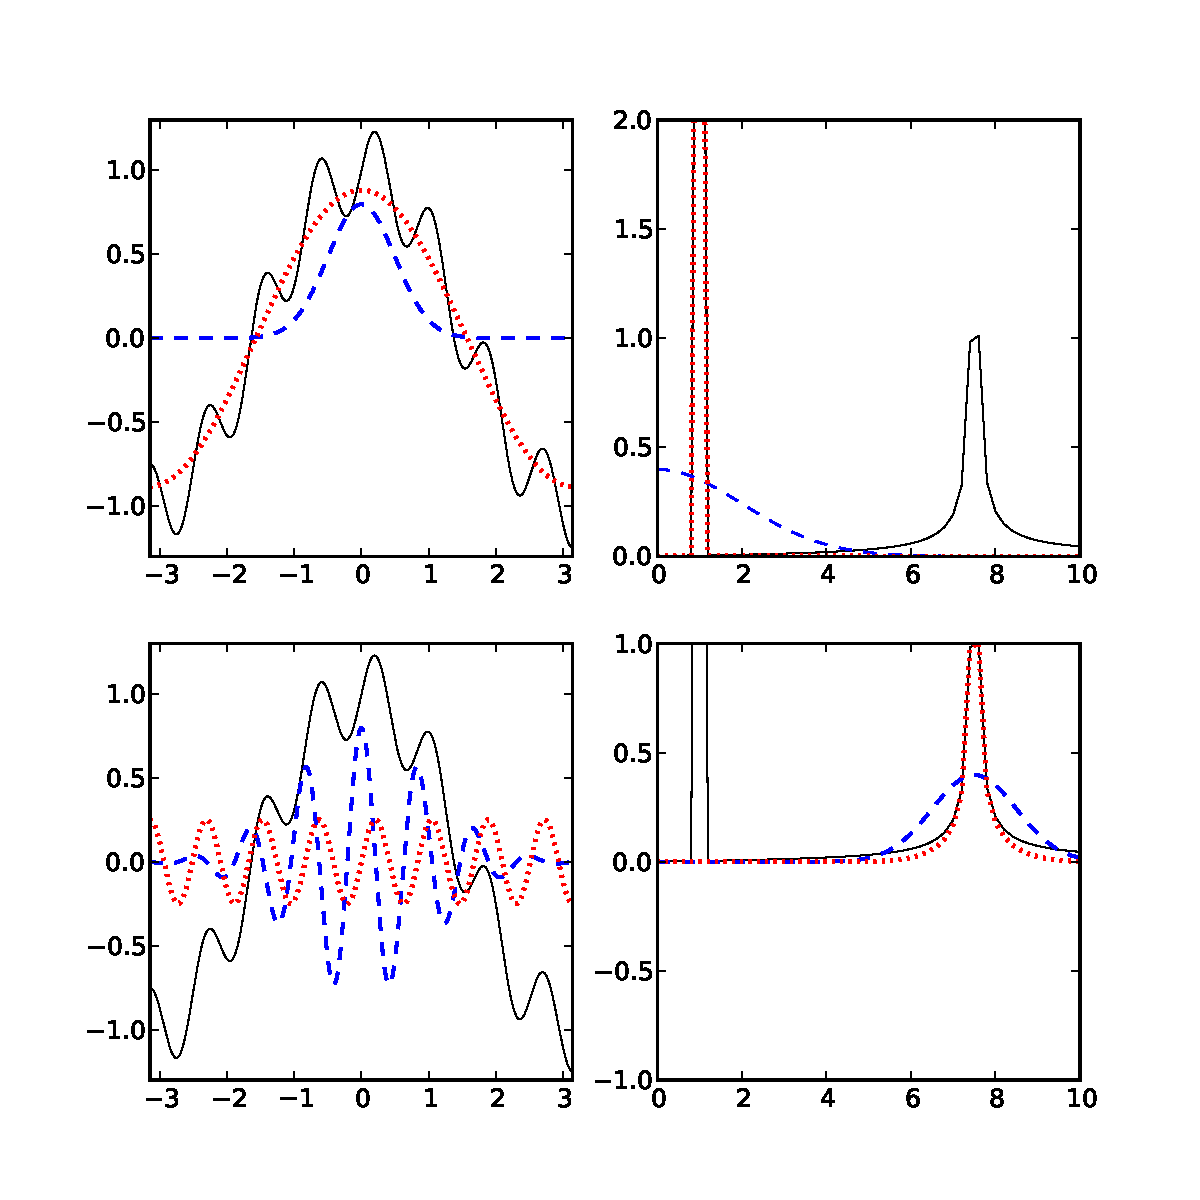
\includegraphics[width=\textwidth]{plots/fouriertrafo}
  \caption{Oben links: Summe zweier Schwingungen $\cos(x) +
    0,25\sin(7,5 x)$ (schwarze Linie), die mit einer Gaußglocke (blau
    gestrichelt) gefaltet wird. Das Ergebnis (rote gepunktete Linie)
    ist die quasi ungestörte langsame Schwingung ohne die
    höherfrequente Schwingung, die weggeglättet wurde. Oben rechts:
    Fouriertransformierte der Funktionen. Klar sichtbar ist die
    hochfrequente Störung mit einer Frequenz von $7,5$, die im
    gefilterten Signal fehlt. In der unteren Reihe wurde eine
    frequenzverschobene Gaußglocke benutzt, um statt der langsamen die
    schnelle Schwingung zu filtern; die Farbcodierung ist wie
    oben. Gemäß \eqref{eq:fourierfreqshift} bewirkt die
    Frequenzverschiebung eine Modulation der Gaußfunktion.}
  \label{fig:fourierfaltung}
\end{figure}

Die Fouriertransformierte der Faltung zweier Funktionen ist
\begin{equation}
  \label{eq:fourierfaltung}
  \begin{split}
    \FT(f\star g)(\omega) &=
    \frac{1}{\sqrt{2\pi}}\int_{-\infty}^{\infty}
    \int_{-\infty}^{\infty} f(t')g(t-t')\,dt' e^{-i \omega t}\,
    dt\\
    &= \frac{1}{\sqrt{2\pi}}\int_{-\infty}^{\infty}
    \int_{-\infty}^{\infty} f(t') g(t) e^{-i \omega (t+t')}\, dt\,
    dt'\\
    &= \frac{1}{\sqrt{2\pi}} \int_{-\infty}^{\infty} f(t')e^{-i
      \omega t'}\, dt' \int_{-\infty}^{\infty} g(t) e^{-i \omega
      t}\, dt = \sqrt{2\pi}\FT(f)(\omega)\FT(g)(\omega).
  \end{split}
\end{equation}
Die Faltung geht also in eine punktweise Multiplikation über. Im
Fourierraum lässt sich also sehr viel schneller falten, als im
Realraum, wo ja für jeden Punkt ein Integral zu lösen ist.

Dies nutzt man auch numerisch, um Faltungen zu berechnen, in
Verbindung mit \eqref{eq:dftcont}. Seien zwei Sätze mit $N$ Datenpunkten $f_k =
f(t_k)$  mit $t_k = t_0 + k\frac{T}{N}$  und $g_k = g(t'_k) $ mit
$t'_k = t'_0 + k\frac{T}{N}$ gegeben. Mit anderen Worten, die beiden
Funktionen müssen mit der selben Frequenz abgetastet worden sein, der
Anfangszeitpunkt kann aber verschieden sein. Das ist etwa beim
Glätten wichtig, bei dem die Filterfunktion meist symmetrisch um die
Null definiert ist, die zu glättende Funktion aber beliebig liegen
kann. Es gilt
\begin{multline}
  \label{eq:discretefold}
  (f\star g)(t_k) =
  \sqrt{2\pi}\FT^{-1}\left(\FT(f)(\omega)\FT(g)(\omega)\right)(t_k)\\
  \approx
  iDFT\left(2\pi \frac{N}{T} \left(e^{i\omega_0 t_0}\right)^n
  \left[\frac{T^2}{2\pi N^2}\left(e^{-i\omega_0 t_0}\right)^n\text{DFT}(f_k)_n\left(e^{-i\omega_0 t'_0}\right)^n\text{DFT}(g_k)_n\right]\right)_k\\
  =
  \frac{T}{N} \text{iDFT}\left[\left(e^{-i\omega_0 t'_0}\right)^n DFT(f_k)_n DFT(g_k)_n\right]_k.
\end{multline}
Wie im Abschnitt~\ref{sec:contdft} besprochen, muss $n$ als Frequenz
im Bereich $-N/2$ bis $N/2$ interpretiert werden. Man beachte, dass
der Faktor $\left(e^{-i\omega_0 t'_0}\right)^n$ nur durch den Aufpunkt
$t'_0$ der Abtastung der Funktion $g$ bestimmt ist, da wir an den
Stellen $t_k$ auswerten. Dadurch ist die Funktion $g$ die
Filterfunktion, die auf $f$ angewendet wird. Ist $g$ wie üblich
symmetrisch um Null abgetastet, so ist $\left(e^{-i\omega_0
    t'_0}\right)^n=(-1)^n$. Vergisst man diesen Term, entspricht das
einem impliziten Verschieben der Filterfunktion zur Null hin.
Die Lage $t_0$ der Abtastung der Funktion $f$ kann hingegen beliebig
verschoben sein. Die Faltung wird in jedem Fall natürlich nur im
Abtastbereich der Funktion $f$ berechnet.

\subsection{Filter}
\index{Filter}

Außerdem lässt \eqref{eq:fourierfaltung} noch eine weitere
Interpretation der Faltung der Funktion $g$ mit der Funktion $f$ zu:
Ist $f$ bzw. $\FT(f)$ reellwertig und symmetrisch, so werden die
einzelnen Frequenzkomponenten der Funktion $g$ mit den
Frequenzanteilen von $f$ gestreckt bzw.\ gestaucht, $g$ also
frequenzgefiltert. Man beachte, dass $g$ für die Definition
\eqref{eq:fourierfaltung} nicht quadratintegrabel sein muss, sofern
der Filter $f$ schnell genug abfällt. Insbesondere kann $g$ eine nur
beschränkte, aber nicht abklingende Funktion sein, wie etwa ein
Messsignal.

Durch Wahl einer symmetrischen und reellwertigen
Fouriertransformierten und Rücktransformation lassen sich also
beliebige Frequenzfilter realisieren; in der Praxis wird natürlich
direkt im Fourierraum gefiltert. Später lernen wir die numerische
diskrete Fouriertransformation kennen, die nicht zuletzt wegen dieser
Filtereigenschaften so wichtig ist. Abbildung~\ref{fig:fourierfaltung}
illustriert einen (gaußschen) Tiefpassfilter und einen Bandfilter, die
nur bestimmte Frequenzen passieren lassen. Daher wird beim
Tiefpassfilter die aufgeprägte hochfrequente Schwingung unterdrückt,
beim Hochpassfilter hingegen die an sich dominante langsame
Schwingung.

\subsection{Antwort zeitinvarianter linearer Systeme}
\index{zeitinvariante lineare Systeme}

Eine weitere wichtige Anwendung der Faltung ist die Bestimmung der
Antwort eines zeitinvarianten linearen Systems auf ein beliebiges
Eingangssignal. Einfach zu messen ist typischerweise die Antwort
$A_\theta(t)$ des Systems auf einen Einschaltvorgang, also ein
Eingangssignal der Form
\begin{equation}
  \theta(t) =
  \begin{cases}
    0 & \text{für}\; t < 0\\
    1 & \text{für}\; t \ge 0.
  \end{cases}
\end{equation}
Um daraus die Antwort auf ein beliebiges Eingangssignal zu bestimmen,
schreiben wir das Eingangssignal $f$ als $f = f \star \delta$. Wegen
der Linearität der Faltung und der Systemantwort ist die Antwort auf
das Signal $f$ gegeben durch die Faltung $A_f(t) = f \star A_\delta$
mit der Antwort auf einen $\delta$-Impuls. Diese Antwort wiederum
lässt sich aus der Sprungantwort durch einfach Ableitung erhalten, was
mit Hilfe der Fouriertransformierten sehr bequem zu berechnen ist:
\begin{equation}
  A_f(t) = f \star A_\delta = f \star
  \frac{d}{dt} A_\theta = \sqrt{2\pi} \FT^{-1}\bigl( i\omega \FT(f) \FT(A_\theta)\bigr).
\end{equation}

\section{Kreuz- und Autokorrelation}
\index{Korrelationsanalyse}

Bis jetzt haben wir uns mit der Verarbeitung idealer Signale
beschäftigt, die zu einem gegebenen Zeitpunkt einen prinzipiell
eindeutig vorherbestimmten Wert haben.  Reale Signale sind aber oft
verrauscht, entweder durch Messungenauigkeiten, Bauteiltoleranzen oder
prinzipielle stochastische Prozesse.  Trotzdem möchte man oft wissen,
ob zwei gemessene Signale von einander abhängig, \emph{korreliert},
sind. Zum Beispiel könnte man die Position eines Elektrons und seinen
Spin, die Menge der verkauften Eis- und Sonnencreme, oder auch die
Position eines Pendels zu zwei verschiedenen Zeitpunkten betrachten.
In den beiden letzteren Fällen werden diese im Allgemeinen korreliert,
also abhängig, sein. Allerdings gibt dies keinen Aufschluss über den
dahinterstehenden kausalen Mechanismus. Im Fall des Pendels rührt die
Korrelation daher, dass es sich in kurzer Zeit nicht beliebig weit von
seiner Ausgangsposition bewegen kann. Bei der Eis- und Sonnencreme
wird es vermutlich auch eine Korrelation geben, aber weder erzeugt
Eiscreme Sonnenbrand, noch macht Sonnencreme Lust auf Eis. Allerdings
haben wir Menschen nunmal bei strahlendem Sonnenschein mehr Lust auf
Eis, aber brauchen auch Sonnencreme.

Formal betrachten wir zunächst zwei Observablen $A$ und $B$. Diese
beiden heißen genau dann unkorreliert, falls die Mittelwerte
$\mean{A\cdot B} = \mean{A}\mean{B}$
bzw. $\mean{(A-\mean{A})(B-\mean{B})}=0$ erfüllen.  Im Allgemeinen
wird man aber vielleich nicht erwarten, dass sich die Änderung einer
Observablen unmittelbar in einer anderen niederschlägt, sondern erst
nach einer Zeit $\tau$.  Man betrachtet daher die Korrelation zwischen
$A$ und $B$ mit einem zeitlichen Versatz von $\tau$, die
\emph{\keyword{Kreuzkorrelationsfunktion}}:
\begin{equation}
  \label{eq:crosscorr}
  C(A,B)(\tau) := \mean{A(0)B(\tau)},
\end{equation}
wobei die Signale $A$ und $B$ zeitinvariant sein sollen, so dass der
Zeitpunkt $t=0$ beliebig gewählt sein kann. Für große $\tau$
dekorrelieren die Signale, daher gilt $C(A,B)\to \mean{A}\mean{B}$ für
$\tau\to\infty$. Wird stattdessen die normierte Kreuzkorrelation
$C(A-\mean{A}, B-\mean{B})$ betrachtet, verschwindet dieses also im
Limit $\tau\to\infty$.

$\mean{\cdot}$ bezeichnet in der Physik üblicherweise den
Ensemblemittelwert, also den Mittelwert über alle möglichen
Realisationen des Experiments. Sind nun $A=A(t)$ und $B=B(t)$
zeitliche Messreihen eines zeitinvarianten Systems, so ermittelt man
die Mittelwerte üblicherweise als Zeitmittelwerte, also Integrale über
die Zeit:
\begin{equation}
  \label{eq:crosscorrtime}
  C(A,B)(\tau) = \mean{A(0)\cdot B(\tau)} \stackrel{!}{=}
  \lim_{T\to\infty}\frac{1}{T}\int_{-T/2}^{T/2} A(t)B(t+\tau)\,dt.
\end{equation}
Das Ausrufezeichen soll andeuteten, dass dies eine Annahme ist, denn
die Gleichheit gilt nur genau dann, wenn das System \emph{ergodisch}
ist, \dh\,, dass der Prozess bei einer unendlich langen zeitlichen
Messung alle möglichen Realisationen einmal besuchen wird. Diese
Annahme wird meist gemacht, obwohl die Ergodizität für die meisten
Systeme nicht bewiesen werden kann. Hinzu kommt, dass ja in der Praxis
niemals über beliebig lange Zeiträume gemittelt werden kann. Daher
können auch endliche, aber hohe Energiebarrieren zu einem
systematischen Fehler führen, weil das System im Zeitraum der Messung
nur den Teil des Phasenraums besucht, der von der Energiebarriere
eingeschlossen ist, selbst wenn auch andere Bereiche zulässig wären.

$\mean{A}$ bzw. $\mean{B}$ sind oft gar nicht genau bekannt, und
müssen numerisch durch \mbox{(Zeit--)}Mittelung der Daten bestimmt
werden. Da hier aber normalerweise dieselben Daten zugrunde gelegt
werden, die auch zu Berechnung der Kreuzkorrelation selber genutzt
werden, sind diese notwendigerweise korreliert, was zu kleinen
Abweichungen in der Kreuzkorrelationsfunktion führt. Im häufigen Fall,
dass eine Observable aus Symmetriegründen einen Mittelwert von Null
haben muss, sollte daher auf keinen Fall der numerische gemessene
Mittelwert abgezogen werden, "`um das Ergebnis zu verbessern"'. Diese
übliche Praxis ist falsch, da sie ja erzwingt, dass der letzte
Datenpunkt der gemessenen Kreuzkorrelationsfunktion notwendigerweise
auf $\mean{A}\mean{B}$ abfällt, selbst wenn einfach nur das
Messinterval zu kurz gewählt wurde. Daher führt diese Methode zu einer
Unterschätzung der Langzeitkorrelationen!

In der Praxis sind $A$ und $B$ natürlich nicht als Funktionen bekannt,
sondern nur als diskrete Messungen. Wir nehmen wie üblich an, dass
diese an endlich vielen, äquidistanten Zeitpunkten $k\Delta$,
$k=0(1)N-1$ stattgefunden haben. Die Gesamtmesszeit beträgt also
$T=N\Delta$. Dann ist in Analogie zu \eqref{eq:crosscorrtime}
\begin{equation}
  \label{eq:crosscorrint}
  C(A,B)(\tau) = \mean{A(0)\cdot B(\tau)}
  = \frac{1}{T}\int_{0}^{T} A(t)B(t+\tau)\,dt.
\end{equation}
Da wir die Messwerte nur an diskreten Stellen kennen, erhalte wir die
Näherung
\begin{equation}
  \label{eq:crosscorrnum}
  C(A,B)(k\Delta)\approx
  \frac{1}{N-k}\sum_{l=0}^{N-k}A(l\Delta)B\left((l+k)\Delta\right)
  \quad\text{für}\; k=0(1)N-1.
\end{equation}
Die unterschiedliche Gewichtung $1/(N-k)$ ergibt sich durch die
unterschiedliche Anzahl an Messungen für den Versatz $k$. Für große
Versätze ist die Anzahl der Messungen sehr klein (für $k=N-1$ nur noch
eine), daher muss $k \ll N$ sein. Bei der Diskretisierung des
Integrals kürzt sich der Vorfaktor $1/T$ gegen die Schrittweite, so
dass nur die Anzahl der Messungen eingeht, nicht aber die Länge des
Messintervalls $T$.

Gleichung \eqref{eq:crosscorrnum} ist numerisch allerdings nicht sehr
effizient auszuwerten, da im allgemeinen $2N^2$ viele Operationen
benötigt werden. Auf der anderen Seite ist die
Kreuzkorrelation~\eqref{eq:crosscorrtime} strukturell einer Faltung
sehr ähnlich.  Daher liegt es nahe, auch hier die FFT gemäß
\eqref{eq:discretefold} zur Beschleunigung einzusetzen. Dazu denken
wir uns die Signale $A$ und $B$ außerhalb $[0,T]$ durch Null
fortgesetzt, so dass wir das Integral in \eqref{eq:crosscorrint}
bedenkenlos nach Unendlich erweitern können. Dann ist
\begin{equation}
  C(A,B)(\tau) = \frac{1}{T}\bigl(A \star B(-\cdot)\bigr)(-\tau) =
  \frac{1}{T} \bigl(A(-\cdot) \star B\bigr)(\tau)\,,
\end{equation}
was effizient im Frequenzraum bestimmt werden kann:
\begin{equation}
  \label{eq:crosscorrfft}
  C(A,B)(t) = \frac{\sqrt{2\pi}}{T}\FT^{-1}
  \bigl(\FT(A)(-\omega)\FT(B)(\omega)\bigr) = \sqrt{2\pi}\FT^{-1}
  \bigl(\overline{\FT(A)}\FT(B)\bigr)\,.
\end{equation}
Diskretisiert ergibt sich schließlich
\begin{equation}
  \label{eq:crosscorrnumfft}
  C(A,B)(k\Delta)
  \approx
  \frac{1}{N}\,\text{iDFT}
  \bigl(\overline{\text{DFT}(A)}\,\text{DFT}(B)\bigr)(k)\,.
\end{equation}
Wie oben kürzt sich der Vorfaktor $\frac{1}{T}$ gegen die Schrittweite
des Integrals, so dass nur die Anzahl der Messungen $N$, aber nicht
die Länge des Messintervalls eingehen. Auch der Vorfaktor
$\left(e^{-i\omega_0 t_0}\right)^n$ in \eqref{eq:discretefold}
entfällt, da beide Messungen nach Voraussetzung bei $t_0=0$ beginnen.

Die Berechnung der 2 DFTs sowie der inversen DFT braucht etwa $6 N\log
N$ Operationen, was normalerweise wesentlich weniger als die $2N^2$
der direkten Berechnung ist.  Allerdings werden das Signal und damit
auch $C(A,B)$ durch die Benutzung der DFT implizit mit Periode
$N\Delta$ periodisiert. Daher sollte $C(A,B)(k\Delta)$ nur für $k\ll
N/2$ interpretiert werden. Wie besprochen gilt dies allerdings genauso
auch für die direkte Auswertung nach \eqref{eq:crosscorrnum}, da für
größere $k$ die Anzahl der Messwerte nicht ausreichend ist.

In Python sieht die Berechnung der Kreuzkorrelation so aus:
\begin{lstlisting}
import numpy
import numpy.fft as fft

def kreuzkorrelation(A, B):
    ftA = fft.fft(A).conj()
    ftB = fft.fft(B)
    return numpy.real(fft.ifft(ftA*ftB))/A.shape[0]
\end{lstlisting}

\subsection{Kreuzkorrelation von Signalen}

Analog zu \eqref{eq:crosscorrtime} kann man die Kreuzkorrelation auch
für \emph{endliche} Signale definieren. Für zwei quadratintegrable, reelle
Signale $f$ und $g$ ist in Analogie die Kreuzkorrelationsfunktion
definiert als
\begin{equation}
  C(f,g)(\tau) = \int_{-\infty}^{\infty} f(t)g(t+\tau)\,dt,
\end{equation}
wobei wegen der Quadratintegrabilität auf die Normierung $1/T$ und
damit den Grenzübergang verzichtet wird. Diese Kreuzkorrelation misst
keine Korrelationen im stochastischen Sinne mehr, weil das Integral
nun keine Zeitmittelung mehr darstellt. Stattdessen ist $C(f,g)(\tau)$
in diesem Fall ein Maß dafür, wie sehr sich die Signale $f$ und $g$
mit einem Zeitversatz $\tau$ im Verlauf ähneln. Diese Form der
Kreuzkorrelation zweier Signale ist einer Faltung noch ähnlicher als
das Zeitmittel: Diese Form der
\begin{equation}
  C(f,g)(\tau) = \bigl(f \star g(-\cdot)\bigr)(-\tau) =
  \bigl(f(-\cdot) \star g\bigr)(\tau).
\end{equation}
Sind die Funktionen $f$ und $g$ wieder äquidistant diskretisiert an
Punkten $t_0 + k\Delta$, $k=0(1)N-1$ gegeben, ist die numerische
Näherung analog zu \eqref{eq:discretefold} gegeben durch
\begin{equation}
  C(f,g)(k\Delta)
  \approx
  \frac{T}{N}\,\text{iDFT}
  \bigl(\left(e^{-i\omega_0 t_0}\right)^n\overline{\text{DFT}(A)}\,\text{DFT}(B)\bigr)(k)\,.
\end{equation}
Anders als beim Zeitmittel, aber analog zur Faltung, entfällt hier der
Vorfaktor $T$ nicht.

\begin{figure}
  \centering
  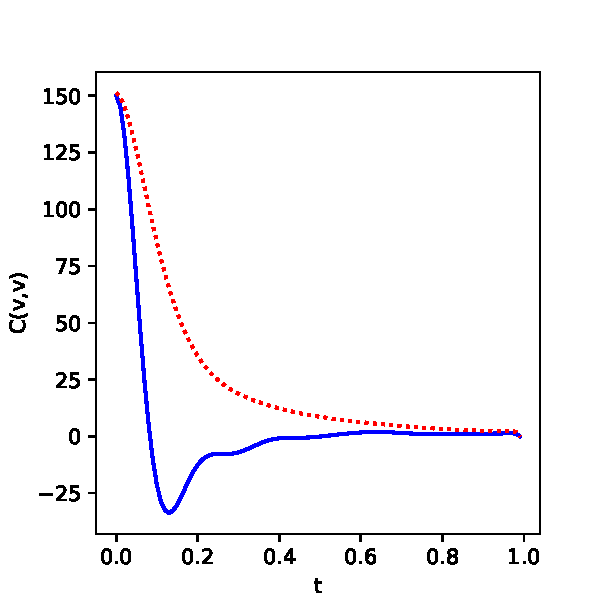
\includegraphics[width=0.5\textwidth]{plots/v_ac}
  \caption{Geschwindigkeitsautokorrelationsfunktion einer temperierten
    Lennard-Jones-Flüs\-sig\-ke\-it mit niedriger Dichte (rot
    gepunktet) und hoher Dichte (blau durchgezogen). Für die niedrige
    Dichte ist die Autokorrelationsfunktion im wesentlichen
    exponentiell abfallend, mit einer Korrelationszeit $\tau_c=0.17$,
    die durch die Kopplungszeit des Thermostaten bestimmt ist.}
  \label{fig:vac}
\end{figure}

\subsection{Autokorrelationsfunktion}

Im Spezialfall $A=B$ spricht man von der
\emph{\keyword{Autokorrelationsfunktion}}. Diese ist offenbar
symmetrisch, daher sind nur Zeitversätze $\tau\ge 0$ von
Interesse. Die Autokorrelationsfunktion misst gewissermaßen, wie lange
es dauert, bis die Observable nicht mehr von ihrem vorherigen Wert
abhängt, wann es diesen sozusagen "`vergisst"'. In dem häufigen Fall,
dass die Autokorrelationsfunktion zunächst exponentiell abfällt, lässt
sich dem Gedächtnis eine Zeitkonstante $\tau_c$, die
\emph{\keyword{Korrelationszeit}}, zuordnen. Diese kann man entweder
durch einen geeigneten Funktionsfit bestimmen, oder aber durch
Integration aus
\begin{equation}
  \label{eq:tauc}
  \int_{0}^{\infty} C(A,A)(\tau)\,d\tau = \int_{0}^{\infty}
  C(A,A)(0)e^{-\tau/\tau_c}\,d\tau = \tau_c\,C(A,A)(0).
\end{equation}

Abbildung~\ref{fig:vac} zeigt die Geschwindigkeitsautokorrelation
$C(v,v)$ einer temperierten Lennard-Jones-Flüs\-sig\-ke\-it bei zwei
verschiedenen Dichten. Die Temperierung wird dabei mit Hilfe eines
Thermostaten erreicht, der die Teilchen stochastisch an ein Wärmebad
koppelt. Dadurch dekorreliert die Geschwindigkeit eines Teilchens in
einer Korrelationszeit von etwa $1/6$.

$C(v,v)$ wird häufig dazu benutzt, um die Diffusionskonstante $D =
\int_0^{\infty} C(v,v)(\tau)\, d\tau$ des Systems zu bestimmen, die
also eng mit der Korrelationszeit des Thermostaten verwandt ist.  Bei
niedriger Dichte ist das System annähernd ein ideales Gas, und die
Teilchen dekorrelieren im wesentlichen nur durch den Einfluss des
Thermostaten, der durch Zufallskräfte wirkt, daher ist $C(v,v)$
tatsächlich gut exponentiell abfallend.  Formel~\eqref{eq:tauc}
bestimmt die Korrelationszeit mit guter Genauigkeit zu etwa
$\tau_c=0.17$, wie durch den Thermostaten zu erwarten. Im Falle der
dichteren Flüssigkeit hingegen kann diese Formel nicht angewendet
werden, da die Autokorrelation kein einfacher exponentieller Abfall
mehr ist, da auch Stoßprozesse eine wichtige Rolle spielen. Diese
führen zum Durchschwingen der Autokorrelationsfunktion.

\section{Messfehlerabschätzung}
\index{Messfehler}

In diesem letzten Abschnitt zur Datenanalyse geht es darum, wie der
Messfehler bei der Messung des Erwartungswerts einer stochastischen
Observable abgeschätzt werden kann. Wir betrachten also eine Messreihe
$x_i$, $i=1(1)N$, die verschiedene Messungen einer stochastischen
Observablen $x$ darstellen, deren Verteilung zeitlich unveränderlich
sein soll (wie zum Beispiel die Temperatur eines abgeschlossenen
Systems im Gleichgewicht). Die gesuchte Größe ist dann meist der
Erwartungswert $\mean{x}$ der Observablen, also der mittlere zu
erwartende Wert der Observablen. Eine einzelne Messung wird im
allgemeinen einen davon abweichenden Wert liefern. Die Größe dieser
Abweichung wird durch die zu erwartende quadratische Abweichung, die
\emph{Varianz}
\begin{equation}
  \sigma^2(x) = \mean{\bigl(x-\mean{x}\bigr)^2}
  = \mean{x^2} - 2\mean{\mean{x}x}  + \mean{x}^2
  = \mean{x^2} - \mean{x}^2,
\end{equation}
beschrieben. Sie ist wie der Erwartungswert eine Eigenschaft der zu
messenden Observablen $x$ und im Gegensatz zum Messfehler nicht von
der Anzahl oder Art der Messungen abhängig. Allerdings lassen sich
weder $\mean{x}$ noch $\sigma^2(x)$ direkt messen, sondern können nur
anhand der Messreihe geschätzt werden.

Der der Erwartungswert lässt sich aus der Messreihe
als
\begin{equation}
  \label{eq:mean}
  \mean{x} \approx \bar{x} := \frac{1}{N}\sum_{i=1}^N x_i
\end{equation}
abschätzen, da offenbar $\mean{\bar{x}} = \mean{x}$. Doch was ist nun der
Fehler, den wir mit dieser Schätzung machen? Dieser ist die zu
erwartende quadratische Abweichung des numerischen Mittelwerts vom
tatsächlichen Erwartungswert:
\begin{equation}
  \mean{\left(\overline{x} - \mean{x}\right)^2} =
  \frac{1}{N^2}\sum_{i,j=1}^N \mean{x_ix_j} -
  \frac{2}{N}\sum_{i=1}^N \mean{x_i}\mean{x} + \mean{x}^2
  = \frac{2}{N^2}\sum_{i > j} \mean{x_ix_j}
  + \frac{1}{N}\mean{x^2} - \mean{x}^2.
\end{equation}
An dieser Stelle nimmt man nun an, dass die Messungen paarweise
unabhängig sind, also, dass $\mean{x_ix_j} = \mean{x_i}\mean{x_j}$ für
$i\neq j$. In der Praxis lässt sich das zum Beispiel durch Betrachten
der Autokorrelationsfunktion sicherstellen, indem nur Messwerte mit
einem zeitlichen Abstand berücksichtigt werden, der sehr viel größer
als die Korrelationszeit ist. Diese Einschränkung werden wir im
folgenden noch genauer untersuchen, für den Moment nehmen wir die
Unabhängigkeit an und erhalten
\begin{equation}
  \label{eq:errestvar}
  \mean{(\overline{x} - \mean{x})^2}
  = \frac{N(N-1)}{N^2}\mean{x}^2 + \frac{1}{N}\mean{x^2} - \mean{x}^2
  = \frac{1}{N}\left(\mean{x^2} - \mean{x}^2\right)
  = \frac{1}{N}\sigma^2(x).
\end{equation}

Als Fehlerbalken wird üblicherweise die \emph{Standardabweichung} der
Messung $\overline{x}$ angegeben. Diese ist durch
\begin{equation}
  \sqrt{\mean{(\overline{x} - \mean{x})^2}}
  = \frac{1}{\sqrt{N}}\sigma(x)
\end{equation}
gegeben. Mit anderen Worten: die Streubreite der Observablen $x$ wird
durch die Mittelung um einen Faktor $1/\sqrt{N}$ gedämpft. Je stärker
$x$ streut, desto mehr Messwerte benötige ich, um den Erwartungswert
zuverlässig abzuschätzen. Für eine Halbierung des Fehlerbalken müssen
bereits viermal soviele Messungen durchgeführt werden, und für eine
Größenordnung an Genauigkeit hundert Mal soviele. Besonders für
Computersimulationen ist das ein Problem, da die Rechenzeit im
allgemeinen proportional zur Anzahl der Messungen ist. Dauert also
eine Simulation eine Woche, was nicht ungewöhnlich ist, so würde eine
Messung mit einer Größenordnung mehr Genauigkeit fast zwei Jahre in
Anspruch nehmen!

Zur Berechnung des Fehlers benötigen wir noch eine Schätzung der
Varianz, die im Allgemeinen ebensowenig wie der Erwartungswert bekannt
ist und geschätzt werden muss. Dazu ersetzt man die Erwartungswerte in
$\mean{x^2} - \mean{x}^2$ durch den Schätzer \eqref{eq:mean}. Für
diesen Ausdruck gilt:
\begin{equation}
  \label{eq:varestalmost}
  \mean{\overline{x^2} - \bar{x}^2}
  = \mean{x^2} - 
  \frac{1}{N^2}\sum_{i=1}^n \mean{x_i^2}
  - \frac{1}{N^2}\sum_{i\neq j} \mean{x_ix_j}
  = \frac{N-1}{N}\left(\mean{x^2} - \mean{x}^2\right),
\end{equation}
wobei wir wieder annehmen, dass die Messungen unabhängig voneinander
sind. Der Ausdruck auf der linken Seite ist selber also \emph{kein} guter
Schätzer für die Varianz, obwohl er genau wie der Schätzer für den
Erwartungswert konstruiert ist. Das liegt daran, dass für die Schätzung
von $\mean{x}$ zweimal $\bar{x}$ und damit zweimal derselbe
Datensatz benutzt wurde.

Ein guter Schätzer für $\sigma^2(x)$ ergibt sich aus der Umkehrung von
\eqref{eq:varestalmost}:
\begin{equation}
  \label{eq:varest}
  \sigma^2(x) \approx \frac{N}{N-1}\left(\overline{x^2} -
    \bar{x}^2\right)
  = \frac{N}{N-1}\left(\overline{(x -
      \bar{x})^2}\right).
\end{equation}
Damit kann für unkorrelierte Daten der quadratische Fehler durch
\begin{equation}
  \label{eq:esterr}
  \mean{(\overline{x} - \mean{x})^2}
  \approx \frac{1}{N}\sigma^2(x)
  = \frac{1}{N-1}\left(\overline{x^2} - \bar{x}^2\right)
\end{equation}
abgeschätzt werden.

Auf dem Computer lassen sich $\mean{x}$ und $\sigma^2(x)$ mit Hilfe
von \eqref{eq:varest} bequem in einem Durchlauf der Daten abschätzen:
\begin{lstlisting}
sum  = 0
sum2 = 0
for v in x:
    sum  += v
    sum2 += v*v
mittel = sum/len(x)
sigma2 = (sum2/len(x) - mittel**2)*len(x)/(len(x)-1)
fehler = sqrt(sigma2/N)
\end{lstlisting}
Der zweite Weg in \eqref{eq:varest} via $\overline{(x - \bar{x})^2}$
ist zwar numerisch etwas stabiler, aber erfordert zwei Schleifen über
alle Daten, da der Mittelwert zunächst bestimmt werden muss, was unter
Umständen zu einer Verdoppelung der Laufzeit führen kann.

Selbstverständlich sind diese elementaren Schätzer aber auch direkt in
NumPy implementiert. \scipy{numpy.mean(x)} berechnet den Schätzer für
den Erwartungswert eines Arrays \argd{x}, \scipy{numpy.var(x, ddof=1)}
den Schätzer für seine Varianz. \argd{ddof} bezeichnet dabei die
Anzahl der abhängigen Freiheitsgrade, die von $N$ im Nenner von
\eqref{eq:varest} abgezogen werden. Wie wir eben gesehen haben, ist
dies bei unabhängigen Daten $\text{\argd{ddof}} = 1$.

\subsection{Fehler bei der Messung korrelierter Daten}

In der Praxis wird oft einfach angenommen, dass die Messungen
unabhängig sind. Was passiert nun, wenn dies nicht der Fall ist?
Betrachten wir also eine Observable die o.B.d.A. Erwartungswert
$\mean{x} = 0$ habe. Dann ist wie oben gezeigt
\begin{equation}
  \label{eq:correrr}
  \mean{(\overline{x} - \mean{x})^2} = \frac{2}{N^2}\sum_{i > j}
  \mean{x_ix_j}
  + \frac{1}{N}\sigma^2(x)
  = \frac{2}{N^2}\sum_{j=1}^{N}\sum_{n = 1}^{N-j} \mean{x_jx_{j+n}}
  + \frac{1}{N}\sigma^2(x).
\end{equation}
Für eine Observable $x$, die in gleichmäßigen Zeitabständen $\Delta$
gemessen wird, lässt sich die innere Summe des linken Terms mit Hilfe
der Autokorrelationsfunktion $C(\tau) = C(x,x)(\tau)$
abschätzen:\nobreak
\begin{equation}
  \sum_{n = 1}^{N-j} \mean{x_jx_{j+n}}
  \approx \int_{n = 0}^{\infty} C(n\Delta)
  = \frac{\tau_\text{int}}{\Delta} C(0)
  = \frac{\tau_\text{int}}{\Delta}\sigma^2(x),
\end{equation}
wobei
\begin{equation}
  \tau_\text{int} := \frac{1}{C(A,A)(0)}\int_0^\infty C(A,A)(\tau)\,d\tau
\end{equation}
die sogenannte \emph{integrierte
  Korrelationszeit}\index{Korrelationszeit>integrierte}
ist. Bei einfachen exponentiellen Prozessen entspricht diese gemäß
\eqref{eq:tauc} genau der klassischen Korrelationszeit
$\tau_c$. Außerdem muss $\tau_\text{int}\ll N\Delta$ sein, so dass die
Erweiterung des Integrals bis unendlich keinen nennenswerten Beitrag
mehr liefert. Eingesetzt in \eqref{eq:correrr} ergibt sich
\begin{equation}
  \label{eq:correrrest}
  \mean{(\overline{x} - \mean{x})^2}
  \approx
  \frac{2}{N^2}\sum_{j=1}^{N} \frac{\tau_\text{int}}{\Delta}\sigma^2(x)
  + \frac{1}{N}\sigma^2(x)
  =
  \left(1 + 2\frac{\tau_\text{int}}{\Delta}\right)\frac{\sigma^2(x)}{N}.
\end{equation}
Der Fehler ist also um einen Faktor $1 + 2 \tau_\text{int} /\Delta$
\emph{größer}, als man aufgrund der Varianz und Anzahl Messungen
erwarten würde, wenn man einfach annimmt, dass die Messungen
unabhängig sind. Setzt man $N_\text{eff} = N \Delta / (2\tau_\text{int})$, dann
ergibt sich
\begin{equation}
  \label{eq:errestvarcorr}
  \mean{(\overline{x} - \mean{x})^2}
  \approx
  \left(1 + 2\frac{\tau_\text{int}}{\Delta}\right)\frac{\sigma^2(x)}{N}.
  \approx \frac{\sigma^2(x)}{N_\text{eff}}.
\end{equation}
Mit anderen Worten, $N_\text{eff}$ kann als die Anzahl der tatsächlich
unabhängigen Messungen interpretiert werden. Nur Messungen, die etwa
zwei Korrelationszeiten auseinanderliegen, sind hinreichend
unabhängig.

Auch der Schätzer \eqref{eq:varest} für die Varianz setzt die
Unabhängigkeit der Messungen voraus. Für abhängige Daten ergibt sich
\begin{align}
  \frac{N}{N-1}\mean{\overline{x^2} - \bar{x}^2}
  &= \frac{1}{N-1}\left(N\mean{x^2} - \mean{x^2}
    - \frac{1}{N}\sum_{i\neq j} \mean{x_ix_j}\right)\nonumber\\
  &= \sigma^2(x) - \frac{2}{N(N-1)}\sum_{i> j} \mean{x_ix_j}
  \approx \left(1 - 2\frac{\tau_\text{int}}{\Delta N}\right)\sigma^2(x).
\end{align}
Die Varianz wird also zusätzlich um einen Faktor $1 -
2\frac{\tau_\text{int}}{\Delta N}$ \emph{unterschätzt}. Immerhin lässt sich
dieser Fehler durch ausreichend viele Messungen minimieren. Allerdings
bringt es nichts, einfach häufiger zu messen, sondern man muss
tatsächlich länger messen, da ja die Gesamtmesszeit $\Delta N$
eingeht.

\begin{figure}
  \centering
  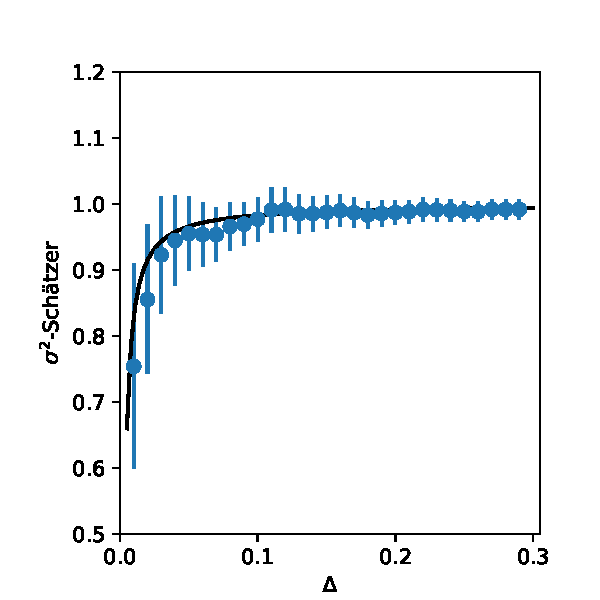
\includegraphics[width=0.5\textwidth]{plots/error}
  \caption{Geschätzte, scheinbare Varianz der Komponenten der
    Geschwindigkeitsverteilung in einem dünnen temperierten
    Lennard-Jones-Systems als Funktion der gewählten Schrittweite
    $\Delta$. Analytisch erwartet man bei der gewählten Temperatur
    eine Varianz von 1. Die blauen Balken geben das
    $1\sigma$-Intervall der beobachteten Varianzen an. Die schwarze
    Linie zeigt die Abschätzung der scheinbaren Varianz gemäß
    \eqref{eq:correrrest} als $(1-2\tau_\text{int}/(\Delta N))\sigma^2(x)$, was
    gut zu den gemessenen Daten passt.}
  \label{fig:error}
\end{figure}

Abbildung~\ref{fig:error} zeigt die scheinbare Varianz der Verteilung
der einzelnen Komponenten der Geschwindigkeit als Funktion der
gewählten Messschrittweite im weniger dichten thermalisierten
Lennard-Jones-System. Diese Geschwindigkeiten sind im thermischen
Gleichgewicht normalverteilt um die Null mit einer Varianz
proportional zur Temperatur des Systems. Im Falle der hier benutzten
Simulationen stellt ein Thermostat sicher, dass die Temperatur exakt 1
ist. Wie man in Abbildung~\ref{fig:error} allerdings deutlich sieht,
wird mit korrelierten Messungen die Varianz, und damit die Temperatur,
um bis zu 25\% unterschätzt, sofern zwischen den Messungen deutlich
weniger Zeit als die Korrelationszeit des Systems, $\approx 0,17$,
liegt. Im Beispiel wurden alle $0,01$ Schritte insgesamt 50.000 Daten
erhoben. Der quadratische Fehler der beobachteten mittleren
Geschwindigkeitskomponenten ist also $1\cdot 34/50.000 \approx 7\cdot
10^{-4}$ anstatt $2\cdot 10^{-5}$, wie man ohne Berücksichtigung der
Korrelationen erhalten würde.

\subsection{Binning-Analyse}
\index{Binning}

Die Messung der integrierten Korrelationszeit $\tau_\text{int}$
ist relativ aufwändig, weil diese die numerische Integration der oft
stark verrauschten Autokorrelationsfunktion erfordert. Eine
Möglichkeit, diese zu umgehen und den Fehler direkt abzuschätzen, ist
die Binning-Analyse~\cite{janke02a}. Diese Methode liefert direkt den
Messfehler, kann aber auch benutzt werden, um $\tau_\text{int}$
abzuschätzen.

Der Ansatz ist naheliegend. Da korrelierte Daten sich auf kurzen
(Zeit-)Abständen nur wenig ändern, ist das Ziel, die Anzahl der Daten
soweit zu reduzieren, dass die verbleibenden Werte gut als unabhängig
angesehen werden können.  Dazu seien die Daten $x$ in $B$ Blöcke
(\enquote{Bins}) der Länge $k$ eingeteilt. Ist $N$ nicht durch $k$
teilbar, muss dazu der Datensatz etwas gekürzt werden, so dass alle
Blöcke voll sind. Anstatt der einzelnen Daten in den Blöcken,
betrachten wir nun nur ihre jeweiligen Mittelwerte
\begin{equation}
  X_{k,l} = \frac{1}{k}\sum_{j=1}^{k}x_{(l-1)k + j}\quad l=1(1)B.
\end{equation}
Offenbar hängen der Erwartungswert und die Varianz der einzelnen
$X_{k,l}$ nicht vom Aufpunkt $l$ ab. Wir schreiben daher kurz $X_k$
für die Observable der Blockmittelwerte der Länge $k$.  Der
Erwartungswert von $X_k$ ist unverändert der von $x$, also $\mean{X_k}
= \mean{x}$, und auch für den Mittelwert aller $X_k$ gilt $\bar{X} =
\bar{x}$. Allerdings ist die Varianz $\sigma^2(X_{k})$ im allgemeinen
von $\sigma^2(x)$ verschieden, und zwar abhängig von $k$. Sofern $k$
sehr viel größer als die typischen Korrelationslängen ist, gilt nach
\eqref{eq:errestvarcorr} $\sigma^2(X_{k}) \approx
\sigma^2(x)/k_\text{eff}$, wobei $k_\text{eff} = k \Delta /
(2\tau_\text{int})$ die effektive Anzahl der unabhängigen Messungen
ist. Für sehr kleine $k$ hingegen spielt die Mittelung keine Rolle,
daher ist $\sigma^2(X_{k}) \approx \sigma^2(x)$.

Diese Verhalten nutzen wir nun, um den Fehler korrelierter Daten
abzuschätzen. Dazu berechnen wir den quadratischen Fehlerschätzer
\eqref{eq:esterr} für die Blockmittelwerte bei verschiedenen
Blockgrößen $k$:
\begin{equation}
  \epsilon^2(k) := \frac{1}{B - 1} \left(\overline{X_k^2} -
    \overline{X_k}^2\right) \approx \frac{k}{N} \sigma^2(X_k).
\end{equation}
Ist $k$ klein, so ist $\sigma^2(X_k)\approx \sigma^2(x)$, und
$\epsilon^2(k)$ wächst linear in $k$. Für große $k$ hingegen ist
$\sigma^2(X_k) \approx \sigma^2(x)/k_\text{eff}$, so dass
$\epsilon^2(k)$ konstant wird, und zwar
\begin{equation}
  \epsilon^2(k)= \frac{k}{N}\frac{\sigma^2(x)}{k_\text{eff}} =
  \frac{\sigma^2(x)}{N_\text{eff}}.
\end{equation}
Der konstante Wert bei großen $k$ ist also der gesuchte tatsächliche
Fehler!  Allerdings stehen bei großen $k$ für die Mittelung immer
weniger Blöcke zur Verfügung, so dass $\epsilon^2(k)$ stark
verrauscht. Daher funktioniert diese Analyse nur, sofern man genügend
Daten gesammelt hat. Auch die Umkehrung gilt: trägt man
$\epsilon^2(k)$ gegen $k$ auf und sieht kein Plateau bei großen $k$,
hat man noch nicht genügend Daten gesammelt, um eine Aussage über die
Güte der Messung zu machen, man benötigt also mehr Daten.

Neben des Fehlers lässt sich für große $k$ auch die integrierte
Korrelationszeit gemäß
\begin{equation}
  \label{eq:tauint}
  k \Delta\frac{\sigma^2(X_k)}{\sigma^2(x)} \approx
  \frac{k\Delta}{k_\text{eff}} = 2\tau_\text{int}
\end{equation}
bestimmen, wobei die Messung von $\sigma^2(x)$ ausreichend unabhängige
Daten voraussetzt. Dies überprüft man zunächst anhand von
$\epsilon^2(k)$.

\begin{figure}
  \centering
  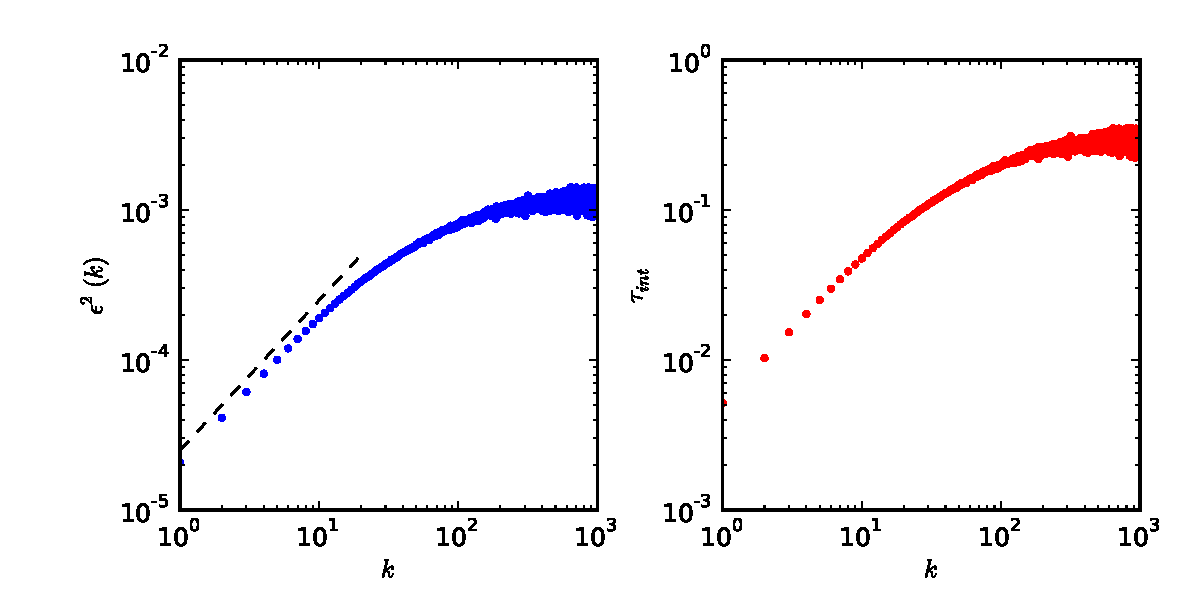
\includegraphics[width=\textwidth]{plots/binning}
  \caption{Links: geschätzter quadratischer Fehler $\epsilon^2(k)$ in
    der Messung der Komponenten der Geschwindigkeitsverteilung in
    einem dünnen temperierten Lennard-Jones-Systems als Funktion der
    Blockgröße $k$. Der Fehler erreicht sein Plateau bei etwa
    0,001, was gut mit der Abschätzung über die Korrelationszeit
    übereinstimmt.  Die gestrichelte schwarze Linie demonstriert das
    lineare Wachstum für kleine $k$. Rechts: Geschätzte integrierte
    Korrelationszeit $\tau_\text{int}$ für dasselbe System.  Diese
    erreicht ihr Plateau bei $\tau_\text{int} \approx 0,25$, was etwas
    größer als das einfach exponentielle $\tau_c\approx 0,17$ ist.}
  \label{fig:binning}
\end{figure}

Abbildung~\ref{fig:binning} demonstriert die Abschätzung des
quadratischen Fehlers und der integrierten Korrelationszeit für
die Messung der Geschwindigkeitskomponenten in der
Lennard-Jones-Flüssigkeit. Wie erwartet werden beide Größen für große
$k$ konstant, aber sind verrauscht, während sie für kleine $k$ linear
anwachsen.  Für die Bestimmung der integrierten Korrelationszeit
wurde das analytische Ergebnis $\sigma^2(x)=1$ benutzt, die gemessene
ist mit $1,03$ etwas größer. Aus der Binning-Analyse ergibt sich ein
quadratischer Fehler von etwa 0,001 und eine integrierte
Korrelationszeit von 0,25, was gut zu unserer Korrelationszeit
$0,17$ und der Fehlerschätzung von $7\cdot 10^{-4}$ passt.

\section{Ausgleichsrechnung, Methode der kleinsten Quadrate}
\index{Ausgleichsrechnung}
\index{Fitting}
\index{Methode der kleinsten Quadrate}

Interpolierende Polynome, Taylorreihen und Splines haben gemeinsam,
das diese möglichst nahe an alle gegebenen Stützstellen verlaufen. Die
Anzahl der Terme in der Approximation ist nur durch die Anzahl der
Stützstellen begrenzt, und meist wählt man so viele Stützstellen wie
möglich, um eine möglichst genaue Näherung der unbekannten
Funktionsform zu erhalten.

Wenn die Daten an den Stützstellen aus Experimenten oder
Computersimulationen gewonnen werden, ist das aber gar nicht
gewünscht, da die Daten selbst nicht exakt sind. Wie wir gesehen
haben, kann deren Qualität zwar durch Mittelung verbessert werden,
trotzdem bleibt eine gewisse Unsicherheit.  Andererseits hat man in
diesem Fall üblicherweise eine Vorstellung aus der Theorie, welche
funktionelle Form die Daten annehmen, und möchte nun wissen, bei
welcher Parameterwahl diese Funktion am besten mit den Daten
verträglich ist. Man möchte also den Parametersatz bestimmen, der den
Abstand der Daten von der Funktion minimiert. Dabei ist bei sinnvollen
Experimenten die Anzahl der Datenpunkte sehr viel größer als die
Anzahl der Parameter.

Seien also wieder Daten $(x_i, y_i)$, $i=0(1)n-1$ und eine Funktion
$f_v(x)$ gegeben. Gesucht ist dann derjenige Parametervektor $v$, der
die Abweichung
\begin{equation}
  \label{eq:leastsq}
  \Delta(v) = \sum_i (f_v(x_i) - y_i)^2
\end{equation}
minimiert. Dieses Verfahren wird auch Methode der kleinste Quadrate
genannt, da ja die quadrierten Abweichungen minimiert werden
sollen. Ist $f_{a,b}(x) = ax + b$ eine Gerade, spricht man auch von
\emph{linearer Regression}\index{lineare Regression}. In diesem Fall lässt
sich das Optimum einfach bestimmen, da
\begin{equation}
  0 = \frac{d}{da} \Delta(a,b) = \sum_i 2 (a x_i + b - y_i)x_i
  = 2n \left(a  \overline{x_i^2} + b \overline{x_i} -
    \overline{y_ix_i} \right)
\end{equation}
und
\begin{equation}
  0 = \frac{d}{db} \Delta(a,b) = \sum_i 2 (a x_i + b - y_i)
  = 2n \left(a  \overline{x_i} + b - \overline{y_i} \right),
\end{equation}
wobei $\overline{x} = \frac{1}{n} \sum_{i=0}^{n-1} x_i$ den Mittelwert
über alle Datenpunkte bedeutet. Daraus ergibt sich
\begin{equation}
  a = \frac{\overline{y_ix_i} -
    \overline{y_i}\cdot\overline{x_i}}{\overline{x_i^2}-\overline{x_i}^2}
  \quad\text{und}\;
  b = \overline{y_i} - a \overline{x_i},
\end{equation}
was sich einfach auf dem Computer berechnen lässt.

\begin{figure}
  \centering
  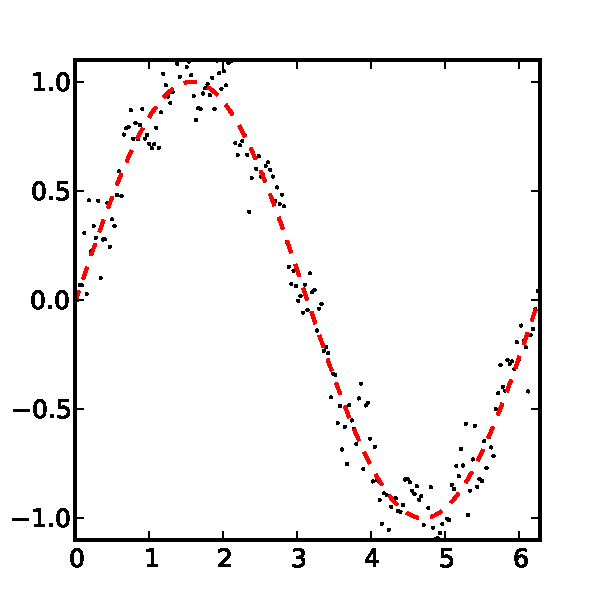
\includegraphics[width=0.5\textwidth]{plots/leastsq}
  \caption{Methode der kleinsten Quadrate zum Fitten der Sinusfunktion
    $y=\sin(x)$. 200 Datenpunkte zwischen 0 und $2\pi$ wurden als
    $\sin(x) + 0,1\,\sin(10 x) + \xi$ erzeugt, wobei $\xi$ eine
    Gauß-verteilte Pseudozufallsvariable mit Varianz $0,01$ war. Die
    resultierende Sinusfunktion (rot gestrichelt) hat die Form $a
    \sin(bx+c)$, wobei die Koeffizienten auf gut 2\% Genauigkeit
    $a=b=1$ und $c=0$ entsprechen. Die kleine höherfrequente
    Schwingung kann durch einen Fit allerdings nicht zuverlässig
    erkannt werden, anders als durch eine Fouriertransformation,
    vergleiche Abbildung~\ref{fig:fourieralias}}
  \label{fig:leastsq}
\end{figure}

Auch für quadratische und andere einfache Funktionen lassen sich die
Koeffizienten geschlossen darstellen, aber bei allgemeinen Funktionen
ist dies nicht immer der Fall. Dann muss die nichtlineare
Optimierungsaufgabe \eqref{eq:leastsq} numerisch gelöst werden, was
wir später behandeln werden. Für den Moment genügt uns, dass SciPy die
Funktion \scipy{scipy.optimize.leastsq(delta, v0, (x, y))} dafür
bereitstellt. \argd{(x, y)} sind dabei die Ausgangsdaten, die hier zu
einem Tupel zusammengefasst sind. \argd{v0} ist der Startwert für die
Berechnung, der nicht zu weit vom (unbekannten) Optimum entfernt
liegen darf. \argd{delta} ist eine Python-Funktion, die als Argumente
$v$, $x_i$ und $y_i$ nimmt und $f_v(x_i) - y_i$ zurückliefert.  Da
$f_v(x)$ eine beliebig komplizierte Form annehmen kann, ist diese
Aufgaben im Allgemeinen nicht lösbar, allerdings funktioniert ein
solcher \emph{Fit} für einfache Funktionen meistens recht
gut. Abbildung~\ref{fig:leastsq} zeigt einen solchen Funktionsfit an
eine verrauschte Sinusfunktion, die mit 200 Datenpunkten auf etwa 2\%
genau gefittet werden kann. Man beachte, das der Ausgangswert für den
Fit mit Hilfe der SciPy-Funktion \lstinline!leastsq! $a=0$, $b=1$,
$c=0$ war; beim Startwert $a=0$, $b=0$, $c=0$ bricht das Verfahren
ab. Das zeigt, dass man tatsächlich nicht zu weit vom Optimum starten
kann, was ein gewisses Verständnis der Zielfunktion voraussetzt.

Ist die Funktionsform, die den Daten zugrundeliegt, unbekannt, ist es
normalerweise keine gute Idee, die Form zu raten. Generell sollte auch
die Anzahl der Parameter sehr klein sein, da sich sonst fast alles
"`gut"' fitten lässt ("`With four parameters I can fit an elephant and
with five I can make him wiggle his trunk."' --- J. von Neumann).

Soll aber zum Beispiel für Visualisierungszwecke eine ansprechende
Kurve entlang der Daten gelegt werden, deren tatsächliche Abhängigkeit
unbekannt ist, dann sind \emph{Pad\'e-Funktionen} oft eine gute
Wahl. Diese haben die Gestalt $P(x)/Q(x)$, wobei $P$ und $Q$ zwei
Polynome mit paarweise verschiedenen Nullstellen sind. Üblicherweise
lassen sich schon für niedrige Polynomgrade ansprechende Fits finden,
sofern die Grade der beiden Polynome in etwa gleich gewählt werden.

%%% Local Variables: 
%%% mode: latex
%%% TeX-master: "padc"
%%% TeX-PDF-mode: t
%%% End: 
